\documentclass[a4paper,11pt]{article}
\usepackage[T1]{fontenc}
\usepackage[utf8]{inputenc}
\usepackage[francais]{babel}
\usepackage[top=3cm, bottom=3cm, left=3cm, right=3cm]{geometry}
\usepackage{lmodern}

% Pour avoir de belles url
\usepackage{url}
\urlstyle{sf}
% Pour utiliser des images
\usepackage{graphicx} 
\graphicspath{{img/}}
% Pour utiliser l'index
\usepackage{makeidx}
\makeindex

% couleurs
\usepackage{color}
\definecolor{bleuClair}{rgb}{0,0.4,0.9}
\definecolor{bleuFonce}{rgb}{0,0.3,0.6}
\definecolor{grisFonce}{gray}{0.40}

% Pour mettre du code source
\usepackage{listings}
\lstnewenvironment{PHP}{
  \lstset{
    frame=trBL,
    language=PHP,
    numbers=left,
    basicstyle=\ttfamily,
    keywordstyle=\color[rgb]{0,0,1},
    commentstyle=\color[rgb]{0.133,0.545,0.133},
    stringstyle=\color[rgb]{0.627,0.126,0.941},
    showspaces=false,
    showstringspaces=false,
    morekeywords={class, extends, public, function},
    breaklines=true,
  }
}{}
\lstnewenvironment{HTML}{
  \lstset{
    frame=trBL,
    language=HTML,
    numbers=left,
    basicstyle=\ttfamily,
    keywordstyle=\color[rgb]{0,0,1},
    commentstyle=\color[rgb]{0.133,0.545,0.133},
    stringstyle=\color[rgb]{0.627,0.126,0.941},
    showspaces=false,
    showstringspaces=false,
    breaklines=true,
  }
}{}
\lstnewenvironment{htaccess}{
  \lstset{
    frame=trBL,
    basicstyle=\ttfamily,
    keywordstyle=\color[rgb]{0,0,1},
    commentstyle=\color[rgb]{0.133,0.545,0.133},
    stringstyle=\color[rgb]{0.627,0.126,0.941},
    showspaces=false,
    showstringspaces=false,
    morekeywords={RewriteEngine, RewriteCond, RewriteRule},
    breaklines=true,
  }
}{}
\lstnewenvironment{ini}{
  \lstset{
    frame=trBL,
    language=HTML,
    basicstyle=\ttfamily,
    keywordstyle=\color[rgb]{0,0,1},
    commentstyle=\color[rgb]{0.133,0.545,0.133},
    stringstyle=\color[rgb]{0.627,0.126,0.941},
    showspaces=false,
    showstringspaces=false,
    morecomment=[l]{;},
    breaklines=true,
  }
}{}

\title{MINZ Is Not Zend\\{\small version 1.0}\\\textbf{Documentation\\ {\small en cours de rédaction}}}
\author{Marien Fressinaud}



\makeatletter
\renewcommand\section{\@startsection{section}{1}{\z@}%
	{2cm \@plus -1ex \@minus -.2ex}%
	{2.3ex \@plus.2ex}%
	{\color{bleuClair}\reset@font\Large\bfseries}}

\renewcommand{\subsection}{\@startsection{subsection}{2}{\z@}%
             {-3.25ex\@plus -1ex \@minus -.2ex}%
             {1.5ex \@plus .2ex}%
             {\color{bleuFonce}\normalfont\large\bfseries}}
\makeatother

\begin{document}

\maketitle

%%%%%%%%%%%%%%%%%%%%%%%%%%%%%%%%%%%%%%%%%%%%%%%%%%%%%%%%%%%%%%%
\newpage
\tableofcontents
\newpage
%%%%%%%%%%%%%%%%%%%%%%%%%%%%%%%%%%%%%%%%%%%%%%%%%%%%%%%%%%%%%%%
\section{Fonctionnement général}
\subsection{Principes fondamentaux}
Pour bien commencer cette documentation, il est important de définir ce qu'est MINZ et de délimiter l'usage qu'il est possible d'en faire.\\

MINZ est un \textbf{framework PHP}, c'est-à-dire qu'il propose une architecture particulière pour l'écriture d'application PHP. On peut le voir comme un squelette, et l'application comme les muscles, cerveaux, peau, etc. Ce framework repose lui-même sur la \textbf{modélisation MVC} (pour Model View Controller). Le modèle MVC permet de séparer logiquement les données (un utilisateur avec un nom, un prénom, un mot de passe par exemple), leur représentation (la façon dont on va les afficher) et leur traitement. Cela permet d'avoir une application facile à maintenir.\\

MINZ est fortement inspiré de \textit{Zend Framework}, qui est un autre framework PHP. Bien qu'inspiré, il s'en éloigne par bien des aspects, d'où son nom en clin d'oeil : \textit{MINZ Is Not Zend}. Il se veut notamment bien plus léger et plus facile à mettre en place afin de faciliter le déploiement d'applications MINZ. Si vous connaissez déjà Zend Framework, il est certain que vous y trouverez de nombreuses similitudes, notamment au niveau de l'architecture.\\

J'ai dans l'idée de rendre MINZ ``compatible'' XMPP. C'est-à-dire que la création d'applications reposant sur XMPP sera grandement facilité. Cela pour démocratiser ce protocole très puissant, et surtout très utile.\\

Si vous souhaitez démarrer rapidement dans le domaine des frameworks, je ne peux que vous conseiller de commencer par MINZ ! :)

\subsection{Architecture}
MINZ repose sur trois répertoires principaux :
\begin{itemize}
  \item \texttt{app} : C'est dans celui-ci que tout le code PHP/HTML de l'application sera écrit, vous n'aurez donc à vous préoccuper \textbf{presque} que de celui-ci.
  \item \texttt{lib} : Tout le code du framework en lui-même se trouve ici, en principe vous n'avez pas besoin d'y toucher. Nous verrons plus tard qu'il est possible d'écrire sa propre librairie, qui se retrouvera donc ici.
  \item \texttt{public} : C'est la partie accessible de l'extérieur, on y retrouve le fichier \texttt{index.php} principal qui lance l'application ainsi que les thèmes, les scripts javascript, les images, etc. Nous verrons plus loin qu'il est possible de mettre son contenu à la racine si jamais on ne peut pas faire pointer le nom de domaine sur ce répertoire.
\end{itemize}

Comme dit ci-dessus, le répertoire \texttt{app} est le plus important car c'est celui-ci qui contiendra les contrôleurs, modèles et vues ainsi que d'autres éléments que nous détaillerons plus loin.\\

Un schéma du fonctionnement est sans doute nécessaire pour bien comprendre comment tout cela fonctionne :
\begin{figure}[h]
  \centering
  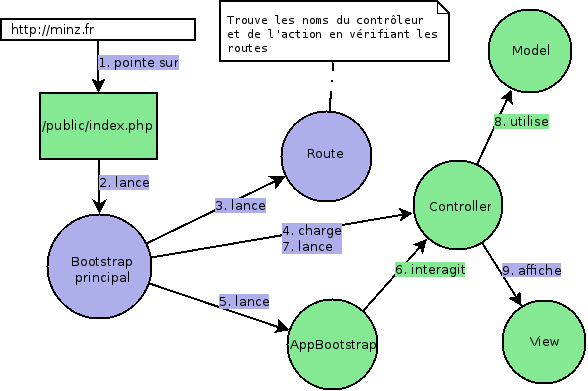
\includegraphics[width=13cm]{schemaFonctionnement.png}
  \caption{Schéma du fonctionnement de MINZ}
  \label{fig1}
\end{figure}

Ce qu'il faut voir ici, c'est l'enchaînement des actions (représentées par les flèches) et comprendre les couleurs. Les ronds représentent des classes PHP. On pourra noter des soucis d'enchaînement (je pense surtout au lancement de la classe Route). Cela devrait être revu dans la version 2 de MINZ, grâce notamment à l'utilisation des \textit{design patterns}.

Les flèches sont numérotées de 1 à 9, et c'est donc l'ordre dans lequel se déroule le fonctionnement du framework. On peut donc voir que lorsque l'url \url{http://minz.fr} est demandée, on va d'abord chercher le fichier \texttt{/public/index.php} qui se charge de lancer le \texttt{Bootstrap}, qui va lui-même demander à récupérer le nom du contrôleur et de l'action à la classe \texttt{Route}, etc.

Pour ce qui est des couleurs, tout ce qui est en bleu représente des classes et méthodes dont vous n'avez pas à vous soucier puisque c'est le framework qui s'en charge lui-même. Tout ce qui est de couleur verte, c'est à vous de le coder. Notez toutefois, si on prend l'exemple du contrôleur, que celui-ci hérite d'une classe parente, donc vous n'avez pas \textbf{tout} à écrire. Si vous avez suivi, en principe, le bleu se trouve dans le répertoire \texttt{lib}, et le vert, dans le répertoire \texttt{app} (à l'exception de \texttt{index.php} qui se trouve dans \texttt{public}).\\

Si tout cela vous paraît un peu obscur, c'est sans doute que mon schéma est mauvais... ou que l'architecture n'est pas terrible... ou les deux ! Il ne tient qu'à vous de me le faire savoir.\\

Par ailleurs, il est important de bien comprendre l'importance de l'action et du contrôleur qui lui est associé. Le framework nécessite de ces deux informations pour fonctionner. Pour cela, on lui indique via l'URL avec la variable \texttt{\$\_GET['c']} le nom du contrôleur à exécuter. La variable \texttt{\$\_GET['a']} sert à donner le nom de l'action. Concrètement, le contrôleur sert à indiquer ce que l'on veut manipuler (par exemple, un Utilisateur) et l'action, une opération à faire sur ce contrôleur (par exemple, ajouter un Utilisateur en base de données).

\subsection{Pré-requis et installation}
Comme il est indiqué dans le fichier \texttt{README} fourni avec le framework, MINZ ne requiert que de peu de choses. La première est \textbf{un serveur Apache} pour l'hébergement. Il a besoin aussi de \textbf{PHP 5}. Pour le moment, je sais qu'il fonctionne sur PHP 5.2.9 et supérieur, mais je pense que des versions antérieures devraient fonctionner aussi. MINZ n'utilise pas beaucoup de fonctions ``exotiques''. Enfin, activer l'\textbf{URL Rewriting} est recommandé pour pouvoir utiliser correctement le système de routes. Sachez toutefois qu'il n'est pas obligatoire (vous devrez utiliser alors des URLs plus traditionnelles). Tout ceci est expliqué plus loin.\\
Et c'est tout ce que je préconise pour pouvoir utiliser le framework, soit des choses que l'on trouve chez la plupart des hébergeurs.\\

Passons à l'installation. Là encore, c'est assez simple. Pour le moment, vous pouvez trouver le code complet sur la page GitHub dédiée :\\ \url{https://github.com/marienfressinaud/MINZ}\\

Une fois les sources téléchargées, il ne vous reste plus qu'à décompresser l'archive sur votre serveur. Assurez-vous que votre nom de domaine pointe sur le répertoire \texttt{public} et modifiez le nom de domaine dans le fichier de configuration (/app/configuration/application.ini). Rendez-vous sur votre site à partir de votre navigateur, et vous devriez voir apparaître l'application par défaut de MINZ ! Félicitations.\\

\textcolor{grisFonce}{\textbf{Remarque} : il se peut que vous ne puissiez faire pointer votre nom de domaine au bon endroit. Deux solutions s'offrent à vous :
\begin{enumerate}
  \item Coupez/collez le contenu de \texttt{public} dans le répertoire dans lequel pointe votre nom de domaine. Des modifications sont alors à porter aux constantes de chemins dans le contenu de \texttt{index.php}.
  \item Dans le fichier de configuration, lors de la modification du nom de domaine, ajoutez le chemin complémentaire. Vous aurez la ligne \texttt{domain = "http://www.minz.test/public"} par exemple si votre nom de domaine pointe sur le répertoire parent de \texttt{public}.
\end{enumerate}
}

\newpage
%%%%%%%%%%%%%%%%%%%%%%%%%%%%%%%%%%%%%%%%%%%%%%%%%%%%%%%%%%%%%%%

\section{Développer avec MINZ}
\subsection{Bien commencer : comprendre le index.php}
Le code de ce fichier est déjà écrit par défaut dans le framework fourni. Il est toutefois important de le comprendre car c'est par là que tout commence. Le code que l'on peut trouver est (à quelque chose près) le suivant :
\begin{PHP}
<?php
// Constantes de chemins
define('PUBLIC_PATH', realpath(dirname(__FILE__)));
define('LIB_PATH', realpath(PUBLIC_PATH.'/../lib'));
define('APP_PATH', realpath(PUBLIC_PATH.'/../app'));
define('LOG_PATH', realpath(PUBLIC_PATH.'/../log'));
define('CACHE_PATH', realpath(PUBLIC_PATH.'/../cache'));

// Ajout du repertoire /lib dans l'include_path
set_include_path(get_include_path().PATH_SEPARATOR.LIB_PATH);

// Parametres du lancement de l'application
$params = array(
'config_file' => APP_PATH.'/configuration/application.ini'
);

require_once('Bootstrap.class.php');

$bootstrap = Bootstrap::getInstance($params);
$bootstrap->init(); // lancement de l'application
\end{PHP}

Le principe ici est d'abord de définir des constantes pour les différents chemins pour faciliter leur utilisation. Ensuite, nous ajoutons notre chemin de librairie à l'\texttt{include\_path} afin de pouvoir inclure les fichiers de librairie en indiquant simplement leur nom plutôt que leur chemin complet.\\

Le chemin vers le fichier de configuration est défini dans un tableau de paramètres. On pourra imaginer dans le futur ajouter d'autres informations à ce tableau.\\

Enfin, on lance le \texttt{Bootstrap}. Tout cela est plutôt simple et ne devrait pas poser de problème mais je pense qu'il est important d'en parler, ne serait-ce que pour avoir connaissance des constantes de chemins qui sont très utiles.

\subsection{Tour d'horizon du répertoire application}
Le répertoire \texttt{app} regroupe à peu près tous les fichiers que vous aurez à écrire. Son contenu est principalement du PHP, mais contient aussi du HTML pour les vues (l'extension est en fait .phtml pour pouvoir utiliser un peu de PHP à l'intérieur quand même). On y retrouve
\begin{itemize}
  \item le répertoire \texttt{configuration} qui contient le fichier de configuration mais aussi le fichier décrivant les routes (nous y reviendrons après)
  \item le répertoire \texttt{controllers} regroupe les contrôleurs de l'application
  \item le répertoire \texttt{models} regroupe les modèles de l'application (y compris ceux permettant d'accéder à la base de données, et autres systèmes de persistance)
  \item le répertoire \texttt{views} regroupe les vues de l'application. À l'intérieur, les vues sont regroupées par contrôleurs et nommées selon l'action qu'elle représente. Ainsi, la vue associée à l'action \texttt{login} du contrôleur \texttt{utilisateur} est representée sur le système de fichier par\\\texttt{/app/views/utilisateur/login.phtml}.
  \item le répertoire \texttt{layout} contient le squelette HTML du site.
  \item le fichier \texttt{AppBootstrap.php} est le Bootstrap de l'application lui permettant d'automatiser un certain nombre d'actions à son lancement.
\end{itemize}

\subsection{Configurer avant de démarrer}
Une étape importante (et indispensable !) est la configuration. Minz propose deux modes de configuration : le fichier .ini et les constantes globales. Je ne peux que vous conseiller que d'utiliser le fichier .ini ! Voilà les différentes options configurables :
\begin{ini}
[general]
; autres valeurs possibles : production / silent (obligatoire)
environment = "development"
; si vous souhaitez utiliser l'url rewriting (obligatoire)
use_url_rewriting = true

; le chemin d'acces a votre application Minz
domain = "http://www.minz.test/public"
; le nom de votre application
title = "MINZ Is Not Zend"
; si vous souhaitez utiliser le layout ou non
layout = true
; la langue par defaut de l'application
language = "fr"
; le nombre d'urls sauvegardees dans l'historique de Minz
max_history_urls = 10
; active ou non le cache
cache_enabled = false

; configuration de la base de donnees
[db]
host = "localhost"
user = "john"
password = "doe"
base = "test"
\end{ini}

Chacune de ces informations sont accessibles à travers la classe \texttt{Configuration}. Les méthodes d'accès sont les suivantes :
\begin{PHP}
public static function environment()
public static function domain()
public static function title()
public static function use_layout()
public static function use_url_rewriting()
public static function data_base()
public static function language()
public static function maxHistoryUrls()
public static function cacheEnabled()
public static function delayCache()
\end{PHP}

\subsection{Écrire un Controller}
Tout d'abord, la norme pour les fichiers de contrôleurs veut que ceux-ci se trouvent dans le répertoire \texttt{/app/controllers} et que leur nom soit de la forme \texttt{nomController} (où \texttt{Controller} est commun à tout contrôleur). Attention à ce que la casse (majuscule/minuscule) corresponde entre le nom de fichier, le paramètre \texttt{\$\_GET['c']} de l'URL et le nom de classe.\\

Le code minimal d'un contrôleur est très simple :
\begin{PHP}
<?php   
class indexController extends Controller {
  public function indexAction() {}
}
\end{PHP}

Il y a deux trois choses à noter ici.\\

Le nom de la classe est ici le nom que l'on passera par l'URL (à l'aide de la variable \texttt{\$\_GET['c'])}.\\

De plus, notre contrôleur hérite de la classe \texttt{Controller}. Cela induit quelques petits éléments, notamment l'accès à la \texttt{View} à travers l'attribut \texttt{\$this->view}. Nous verrons dans la partie suivante les actions que l'on peut lui appliquer. Ensuite, les méthodes \texttt{firstAction()} et \texttt{lastAction()} peuvent être redéfinies. Ce sont des actions qui vont se lancer avant et après chacune des actions que vous allez écrire par la suite pour ce contrôleur particulier.\\

Enfin la méthode \texttt{indexAction} correspond à l'action \texttt{index} (l'action par défaut pour tout contrôleur). Vous aurez donc à écrire d'autres actions. Celles-ci se lanceront en fonction du paramètre \texttt{\$\_GET['a']} passé dans l'URL. Vous pourrez manipuler la vue à l'intérieur de ces méthodes. Par exemple, si votre méthode correspond à l'accueil de votre site, vous pouvez ajouter un titre comme ceci :
\begin{PHP}
public function indexAction() {
  $this->view->appendTitle('Accueil - ');
  // ou
  $this->view->prependTitle(' - Accueil');
}
\end{PHP}

La syntaxe sera expliquée plus loin mais est tout de même simple à comprendre.\\

Ainsi, dans ces méthodes, vous pouvez aussi manipuler les \texttt{Models} qui permettront d'accéder à la base de données et les transmettre à la vue pour que celle-ci les affiche.

\subsection{Écrire une View}
Il est important de comprendre que les Views s'utilisent de deux manières complémentaires. Tout d'abord à l'intérieur des Controllers, puis ensuite dans les fichiers de type .phtml qui décrivent le code HTML.\\

Dans un contrôleur, nous l'avons vu, la vue est accessible à l'aide de l'attribut \texttt{\$this->view}. On peut lui ajouter des variables très facilement de cette manière : \texttt{\$this->view->maChaine = 'ma super chaine';}\\
Ici il s'agit d'une chaîne, mais bien sûr il peut s'agir de tout type de variable, et le plus souvent il s'agira d'objets contenant les données à manipuler, issues de la base de données. De cette manière vous pouvez transmettre facilement des données à la vue.\\

À noter qu'il existe plusieurs méthodes applicables sur une \texttt{View} qui permettent notamment d'ajouter des fichiers CSS et des scripts javascript. Le détail est donné plus loin.\\

Ensuite, l'affichage des vues se fait à l'aide de code HTML. À noter qu'une vue correspond à une action donnée, correspondant elle-même à un contrôleur donné. Ainsi le nommage se fera de cette manière : \\\texttt{/app/views/controller/action.phtml} où \textbf{controller} correspond au nom du contrôleur concerné, et \textbf{action} à l'action concernée.\\
Le contenu de ces fichiers sera du HTML mais vous pouvez tout de même y utiliser du PHP, notamment pour manipuler les données. À noter que lorsque vous travaillez dans ces fichiers vous êtes \textbf{dans} la vue, c'est-à-dire que les variables qui étaient accessibles tout à l'heure à travers \texttt{\$this->view->variable} dans le contrôleur, seront accessibles directement : \texttt{\$this->variable}. Ainsi un contenu possible, en reprenant l'exemple de la chaîne de tout à l'heure, sera :
\begin{HTML}
<div id="header"><?php echo $this->title; ?></div>
<p><?php echo $this->maChaine; ?></p>
\end{HTML}

qui affichera deux blocs affichant d'abord le titre de l'application, puis le paragraphe ``\textit{ma super chaîne}''.

\subsection{Écrire un Model}
Le modèle dit "de base" est le coeur de l'application. C'est lui qui représente les éléments "métier". Ainsi le modèle pourra représenter un utilisateur, un article de blog, une photo d'une galerie. On peut appliquer à chacun de ces modèles des actions : par exemple, l'utilisateur possédera une méthode \texttt{login()} qui lui permettra de se connecter.\\
Tout modèle doit étendre la classe \texttt{Model}.

\begin{PHP}
class User extends Model {
  private $username;
  private $mail;

  public function __construct($username, $mail) {
    $this->username = $username;
    $this->mail = $mail;
  }

  public function login($username, $password) {
    // dans un cas reel, on ira verifier les infos en base de donnees
    if($username=='john' && $password=='doe') {
      // attribue $username a une variable de session
      Session::_param('username', $username);
    }
  }

  public function isLogged() {
    // permet de recuperer la variable de session 'username'
    $username = Session::param('username');

    return !empty($username);
  }
}
\end{PHP}

Le modèle de base est très utile, mais bien souvent insuffisant, surtout dans une application web qui stocke des données. En effet, on aura bien souvent besoin de sauvegarder une liste d'utilisateurs en base de données (par exemple). Ainsi, le modèle DAO va permettre d'accéder à ces informations. À ce jour, 3 modes d'accès à des supports de stockage sont disponibles dans MINZ : les fichiers textes, les tableaux PHP (stockés dans des fichiers texte) et les bases de données MySQL (utilisant PDO)

\begin{PHP}
// La connexion a la BDD se fait automatiquement grace aux infos donnees dans le fichier de configuration
// a inclure avec include_once(APP_PATH.'/models/dao/UserDAO.sql.php'); dans User.php
class UserDAO extends Model_sql {
  public function searchByUsername($username) {
    $sql = 'SELECT * FROM user WHERE loginUser=?';
    
    $stm = $this->bd->prepare($sql); 
    $stm->execute(array($username));
    $res = $stm->fetchAll(PDO::FETCH_CLASS);
    
    if(isset($res[0])) {
      return $res[0];
    } else {
      return false;
    }
  }
}
\end{PHP}
%$

Notre problème ici est que nous renvoyons une classe "non connue" par l'application et tirée de la base de données. Une bonne pratique est de "mapper" cet objet "BDD" avec un modèle déjà écrit afin que le modèle DAO ne renvoie que des modèles "User", codé plus haut. Pour cela nous allons utiliser un Helper :

\begin{PHP}
class HelperUser {
  // permet de convertir un Model DAO (tire de BDD ici) en Model
  // on peut aussi creer une methode convertissant des listes de Model DAO
  public static function daoToUser($dao) {
    return new User($dao->loginUser, $dao->mailUser);
  }
}
\end{PHP}

Ainsi, nous utiliserons cette méthode dans la classe UserDAO en remplaçant
\begin{PHP}
return $res[0];
\end{PHP}
par
\begin{PHP}
return HelperUser::daoToUser($res[0]);
\end{PHP}
En pensant bien à inclure le fichier de Helper dans UserDAO
\begin{PHP}
include_once(APP_PATH.'/models/helper/HelperUser.php');
\end{PHP}

\subsection{Lier le tout}
Maintenant que nous avons vu chacun des modules important, il est tant d'articuler tout ça autour d'un contrôleur concret. Nous allons donc réutiliser les modèles écrits jusque-là. Cet exemple permet de rechercher dans une base de données un utilisateur, à partir d'un username passé via l'url.\\

Le contrôleur
\begin{PHP}
include(APP_PATH.'/models/User.php');

class indexController extends Controller {
  public function indexAction() {
    // recupere le username dans l'url (variable $_GET['username'])
    // on met $username = 'john' par defaut
    $username = Helper::fetch_get('username', 'john');
  
    // recherche en BD de l'utilisateur
    $userDAO = new UserDAO();
    // si non trouve, retourne false
    $this->view->user = $userDAO->searchByUsername($username);
    
    // On change quelques infos sur la page
    $this->view->appendTitle("Recherche d'un utilisateur - ");
    // url permet de gerer facilement les urls internes a l'application MINZ
    // son utilisation sera decrite plus loin
    $this->view->prependStyle($this->view->url->display().'/theme/defaut.css');
  }
}
\end{PHP}

La vue
\begin{HTML}
<!DOCTYPE html>
<html>
  <head>
    <?php echo $this->headTitle(); ?>
    <?php echo $this->headStyle(); ?>
  </head>
  <body>
    <h1><a href="<?php echo $this->url->display();?>"><?php echo $this->title; ?></a></h1>

    <?php if(!$this->user) { ?>
    <p class="error">L'utilisateur recherche n'existe pas.</p>
    <?php } else { ?>
    <p class="infos">L'utilisateur <?php echo $this->user->username(); ?> possede l'adresse mail <?php echo $this->user->mail(); ?>.</p>
    <?php } ?>
  </body>
</html>
\end{HTML}
%$

\subsection{Utilisation d'un layout}
Dans l'exemple précédent, nous avons vu qu'il fallait mettre tout le code HTML dans la vue associée à l'url. Cependant, très vite, recopier l'ensemble de la structure HTML dans toutes les vues va devenir long et fastidieux. Et c'est sans compter la maintenance du code qui va vite devenir insupportable.

Nous allons donc voir le fonctionnement du principe du Layout qui permet de définir une structure globale à l'application dans laquelle viendra se greffer simplement le code spécifique aux vues.\\

Tout se passe maintenant dans le dossier /app/layout. Le fichier de base est \texttt{layout.phtml}. On peut y mettre ainsi tout le code HTML global à l'application. En se basant sur l'exemple précédent, nous aurons donc :
\begin{HTML}
<!DOCTYPE html>
<html>
  <head>
    <?php echo $this->headTitle(); ?>
    <?php echo $this->headStyle(); ?>
  </head>
  <body>
    <h1><a href="<?php echo $this->url->display();?>"><?php echo $this->title; ?></a></h1>

    <?php $this->render(); ?>
  </body>
</html>
\end{HTML}
%$

La méthode \texttt{render()} associée à la classe View permet d'afficher la vue spécifique à l'url demandée.

On aimerait aussi pouvoir mieux départager les différentes grandes parties de la structure. Ainsi ici le titre qui est global à toute l'application pourrait être séparé dans un fichier à part (\texttt{title.phtml} par exemple). Cela est possible grâce au principe des partials. Notre code ressemblera donc à ça maintenant : 

/app/layout/layout.phtml
\begin{HTML}
<!DOCTYPE html>
<html>
  <head>
    <?php echo $this->headTitle(); ?>
    <?php echo $this->headStyle(); ?>
  </head>
  <body>
    <?php $this->partial('title'); ?>

    <?php $this->render(); ?>
  </body>
</html>
\end{HTML}

/app/layout/title.phtml
\begin{HTML}
<h1><a href="<?php echo $this->url->display();?>"><?php echo $this->title; ?></a></h1>
\end{HTML}

Et la vue
\begin{HTML}
<?php if(!$this->user) { ?>
<p class="error">L'utilisateur recherche n'existe pas.</p>
<?php } else { ?>
<p class="infos">L'utilisateur <?php echo $this->user->username(); ?> possede l'adresse mail <?php echo $this->user->mail(); ?>.</p>
<?php } ?>
\end{HTML}
%$

\subsection{Utiliser l'AppBootstrap}
Notre application va grossir, on va devoir ajouter des actions au contrôleur, des contrôleurs à l'application, etc. Et un problème va vite se faire sentir : qu'en est-il de la duplication de code ? Par exemple, la feuille de style que l'on doit ajouter dans chaque contrôleur ne pourrait-elle pas être ajoutée une bonne fois pour toute ?

C'est là qu'intervient l'\texttt{AppBootstrap}. Ce mécanisme permet d'automatiser certaines tâches répétitives. Pour se faire, rien de plus simple : il suffit de créer le fichier /app/AppBootstrap.php et d'y ajouter le code suivant (obligatoire)
\begin{PHP}
class AppBootstrap {
  private $view;

  public function __construct() {
    $controller = Controller::getInstance();
    $this->view = $controller->getView();
  }

  // Fonction lancee par le Boostrap de la librairie et permet de charger les elements redondants dans chaque Controller.
  public function run() {}
}
\end{PHP}

Il ne vous reste plus alors qu'à ajouter ce qu'il vous faut dans la méthode \texttt{run()}. Notez que tout ce qu'il est possible de faire dans un contrôleur, est possible dans l'AppBootstrap. Il vaut mieux cependant s'en tenir au strict minimum. Par exemple :
\begin{PHP}
public function run() {
  include(APP_PATH.'/models/User.php');
  $this->view->prependStyle($this->view->url->display().'/theme/defaut.css');
}
\end{PHP}


\subsection{Router les URLs}
Ok, nous avons une application qui tourne à peu près correctement. Malheureusement, comme nous l'avons vu, le contrôleur et l'action à exécuter passe via les paramètres renseignés dans l'url. Du coup celle-ci n'est pas très jolie :( Par exemple, l'url pour accéder à un article de blog pourrait être de la forme \url{http://votre-domaine.fr/?c=blog&a=voir&id=42}

Heureusement, l'url rewriting est là pour vous ! Ici, nous n'allons pas vraiment voir ce que nous propose Apache car ce n'est pas le but (et je n'ai jamais trouvé ça facile !). Aussi, la seule chose que vous avez à faire dans votre fichier \texttt{.htaccess} est d'ajouter ces lignes :
\begin{htaccess}
RewriteEngine On
RewriteCond %{REQUEST_FILENAME} -s [OR]
RewriteCond %{REQUEST_FILENAME} -l [OR]
RewriteCond %{REQUEST_FILENAME} -d
RewriteRule ^.*$ - [NC,L]
RewriteRule ^.*$ index.php [NC,L]
\end{htaccess}

Cela permet tout simplement de rediriger toutes les requêtes tombant sur votre site sur le fichier index.php, laissant la main ainsi au framework. Assurez-vous maintenant que la variable \texttt{use\_url\_rewriting} dans le fichier de configuration soit bien à \texttt{true}.

Le principe de l'url rewriting dans Minz repose sur un tableau PHP associant 3 ou 4 éléments :
\begin{itemize}
  \item la \texttt{route} qui correspond à l'url amenant à la page demandée
  \item le contrôleur associé à cette route
  \item l'action associée elle aussi à cette route
  \item et un tableau de paramètres supplémentaires pour pouvoir utiliser des urls dynamiques
\end{itemize}

Aussi, vu qu'un exemple est plus parlant que du blabla, voici le contenu d'un fichier /app/configuration/routes.php
\begin{PHP}
return array(
  // blog
  array(
    'route'       => '/blog',
    'controller'  => 'blog',
    'action'      => 'index'
  ),
  array(
    'route'       => '/blog/tag/*',
    'controller'  => 'blog',
    'action'      => 'search',
    'params'      => array('tag')
  ),
  array(
    'route'       => '/blog/*/*',
    'controller'  => 'blog',
    'action'      => 'voir',
    'params'      => array('id','title')
  ),
  array(
    'route'       => '/*',
    'controller'  => 'index',
    'action'      => 'index',
    'params'      => array('page')
    ),
);
\end{PHP}

Ici, nous renvoyons un tableau contenant l'ensemble des règles de réécriture. Chaque règle est définie elle-même dans un tableau. Afin de définir une url dynamique, nous utilisons l'astérisque (*). Attention, celle-ci doit obligatoirement se trouver \textbf{seule} derrière un slash (/). Afin de définir le nom de la variable \texttt{\$\_GET[]}, on l'indique dans le tableau associé à \texttt{params}.

Une petite remarque importante : comme j'ai voulu l'illustrer avec la dernière règle, celle-ci pourrait être confondue avec la première. En effet, "blog" pourrait être mappé avec l'astérisque et être envoyé en tant que valeur de la variable \texttt{\$\_GET['page']}. Pour pallier à ce problème, il faut savoir que Minz s'arrête à la première règle rencontrée correspondant à l'url actuelle. Dans mon exemple, il n'y a donc pas de problème, mais en inversant les deux règles, on ne pourrait plus accéder au contrôleur "Blog" et son action "index". Attention donc à l'ordre de vos règles et faire en sorte qu'elles ne s'écrasent pas les unes les autres.\\

On pourra imaginer un certain nombre d'améliorations possibles au niveau du routage des urls. Le routage dynamique est limité par la séparation obligatoire des variables entre des slashs (/), j'avais commencé à penser à les définir, à la place des astérisques, par des accolades et l'on aurait pu avoir quelque chose de la forme :
\begin{PHP}
array(
  'route'       => '/blog/{id}-{title}.html',
  'controller'  => 'blog',
  'action'      => 'voir'
)
\end{PHP}
Mais ça demande pas mal de changements, et je n'ai jamais pris le temps de le faire. De plus, le problème de l'ordre des règles peux poser quelques problèmes.

\newpage
%%%%%%%%%%%%%%%%%%%%%%%%%%%%%%%%%%%%%%%%%%%%%%%%%%%%%%%%%%%%%%%

\section{Aller plus loin}
Nous avons vu dans la partie précédente toutes les bases de MINZ. Celle qui suit va décrire un peu plus en profondeur quelques aspects "moins importants", mais pratiques au quotidien.

\subsection{Les variables de session}
On l'a déjà un peu vu précédemment, les variables de session sont gérées à travers la classe \texttt{Session}. Cette dernière ne fait que gérer en son sein la variable globale \texttt{\$\_SESSION}. Voyons voir un peu ses spécificités.\\

La session est démarrée automatiquement par le framework, vous n'avez donc pas à vous en inquiéter.
\begin{PHP}
// assigne une valeur a la variable username
Session::_param('username', 'john');

// recupere la valeur
$username = Session::param('username');

// supprime la variable
Session::_param('username', false);
// ou
Session::_param('username');

// efface la session
Session::unset_session();
// ou pour forcer la suppression de l'historique et de la langue
Session::unset_session(true);
\end{PHP}
%$

Comme précisé dans les commentaires, il existe deux variables de session un peu spéciales :
\begin{itemize}
  \item \texttt{history} est un tableau mémorisant l'historique de navigation du visiteur. Utile pour les retours en arrière (mais nécessiterait des améliorations)
  \item \texttt{language} permet de stocker la langue dans laquelle afficher le site. Utile pour internationaliser son application.
\end{itemize}

\subsection{Gérer facilement les urls internes}
Vous aurez peut-être noté que l'url rewriting est facultatif d'usage. Aussi il peut être intéressant de l'activer / désactiver à la volée pour rendre votre application un peu plus portable (vu que nombre d'hébergeurs ne propose pas l'url rewriting).

Problème : comment faire en sorte pour que les liens internes au site soient toujours correctement formatés ?

Il existe pour ça la classe \texttt{Url}, dont une instance est directement accessible à partir de la vue. La seule méthode utilisable est \texttt{display()}, prenant un tableau décrivant l'url en paramètre. Petit exemple (on se situe dans un fichier de vue) :
\begin{HTML}
<a href="<?php echo $this->url->display(); ?>">Un lien vers l'accueil du site</a>

<?php
  $urlBlog = array(
    'c' => 'blog',
    'a' => 'index',
    'params' => array('page'=>2)
  );
?>

<a href="<?php echo $this->url->display($urlBlog); ?>">Un lien vers la page 2 du blog</a>
\end{HTML}

Le gros avantage est que vous n'avez plus à vous soucier du format de vos urls, tout est géré par le framework, que l'url rewriting soit activé ou non.

\subsection{L'historique du parcours de vos utilisateurs}
J'en ai déjà parlé plus haut, vous pouvez gérer l'historique du parcours de vos visiteurs. Malheureusement la classe le proposant devrait être revue car sujette à quelques problèmes.\\

Trois méthodes sont disponibles, mais seulement deux vraiment utiles :
\begin{itemize}
  \item \texttt{put(\$url)} permet d'ajouter une url à l'historique. En principe c'est le framework qui s'en occupe tout seul, vous n'en avez en principe pas besoin.
  \item \texttt{back([\$step[, \$default]])} renvoie par défaut l'url de la page précédente. Vous pouvez spécifier le nombre de pas en arrière à faire ainsi qu'une url par défaut si aucune url n'est trouvée.
  \item \texttt{delete([\$num])} supprime une url. Si rien n'est spécifié, toutes les urls seront supprimées. Vous pouvez l'utiliser pour ne pas sauvegarder la page actuelle (utile lors d'un passage sur une page de redirection par exemple)
\end{itemize}

Un exemple d'utilisation :
\begin{HTML}
<?php 
  $defaut = array(
    'c' => 'index',
    'a' => 'index'
  );
  $urlPrecedente = History::back(History::PREVIOUS_PAGE, $defaut);
?>

<a href="<?php echo $this->url->display($urlPrecedente); ?>">Un lien vers la page precedente</a>
\end{HTML}
%$

\subsection{Utilisation du système de Cache}
Un site peut vite devenir lourd à charger lorsque de nombreuses choses sont faites en amont. Pour ça, il existe le cache. Dans Minz, une fonctionnalité permet de gérer facilement le cache de vos pages web.

Si rien n'est spécifié, à chaque passage sur une page non visitée, celle-ci est enregistré dans le cache (en principe dans le répertoire /cache). À la visite suivante sur cette même page, aucun calcul ne sera fait et Minz se contentera de renvoyer la page du cache.

Un problème se pose si vous êtes connectés avec un compte administrateur et que c'est vous qui enregistrez le cache. Vos visiteurs auront la page de cache avec des liens vers votre administration ! Une bonne pratique est alors de désactiver le cache lorsque vous êtes connectés. Par exemple, dans l'AppBootstrap on pourrait avoir quelque chose de la forme :
\begin{PHP}
$user = new User();

if($user->isLogged()) {
  Cache::switchCache();
}
\end{PHP}

Une autre manière est de désactiver totalement la mise en cache dans le fichier de configuration (\texttt{cache\_enabled = false})\\

L'activation ou non du cache est à peu près la seule chose dont vous avez à vous soucier, tout le reste étant géré par le framework.

\subsection{Internationaliser son application}
Votre site commence à prendre de l'ampleur et vous commencez à lorgner vers une internationalisation de celui-ci ? Tout est prévu !

La classe \texttt{Translate} permet, à partir de fichiers sous la forme 'clé' => 'traduction', de traduire facilement votre application. Si la clé n'est pas présente dans le fichier, la valeur retournée sera la clé elle-même. Ces fichiers se placent dans le répertoire /app/i18n/. Par exemple, deux fichiers :

/app/i18n/fr.php
\begin{PHP}
return array(
  'home' => 'Accueil',
  'welcome' => 'Bienvenue !',
  'connection' => 'Connexion',
}
\end{PHP}

/app/i18n/en.php
\begin{PHP}
return array(
  'home' => 'Home',
  'welcome' => 'Welcome !',
  'connection' => 'Connection',
}
\end{PHP}

Ensuite, pour utiliser ceci, la vue propose une instance de Translate pouvant être utilisé ainsi :
\begin{HTML}
<h2><?php echo $this->translate->t('welcome');?></h2>
\end{HTML}
%$

La langue par défaut peut être définie dans le fichier de configuration (\texttt{language = "fr"} par exemple). Et pour permettre à vos visiteurs de modifier la langue, il suffit de changer la valeur de la variable de session '\texttt{language}' (dont on a parlé plus haut).

Notez que la valeur de cette variable doit être le nom du fichier de traduction (convention Minz).

\subsection{La View en détails}
Il est temps de détailler la classe View un peu plus en profondeur. Voyons donc ses méthodes plus ou moins utiles :
\begin{itemize}
  \item \texttt{render()} utilisé en principe dans le layout pour afficher la vue.
  \item \texttt{renderWithLayout()} vous n'avez en principe pas besoin de l'utiliser, cela permet d'afficher la vue avec le layout.
  \item \texttt{partial(\$file)} affiche un morceau de layout.
  \item \texttt{has\_layout()} permet de savoir si le layout est activé.
  \item \texttt{switchLayout()} permet de switcher l'utilisation du layout.
  \item \texttt{headTitle()} retourne le titre de l'application dans la balise html \texttt{<title>}
  \item \texttt{headStyle()} retourne la liste des fichiers css (assez limité)
  \item \texttt{headScript()} retourne la liste des scripts javascript (assez limité)
  \item \texttt{setTitle(\$title)} change le titre de l'application
  \item \texttt{appendTitle(\$title)} ajoute un titre \textbf{avant} le titre actuel (même principe pour \texttt{appendStyle} et \texttt{appendScript})
  \item \texttt{prependTitle(\$title)} ajoute un titre \textbf{après} le titre actuel (même principe pour \texttt{prependStyle} et \texttt{prependScript})
\end{itemize}

\subsection{Paginer les longues listes}
Imaginons une liste d'une vingtaine d'articles de blog. Vous aimeriez bien paginer cette liste sur différentes pages afin de ne pas tout afficher tout d'un coup. Nous avons pour se faire la classe \texttt{Paginator}.

Dans le contrôleur
\begin{PHP}
// recupere le numero de page actuel
$page = Helper::fetch_get('page', 1);
// cree un paginator en prenant en parametre un tableau
$this->view->articlesPaginator = new Paginator($articles);
// indique le nombre d'article a afficher
$this->view->articlesPaginator->_nbItemsPerPage(5);
// indique la page actuelle
$this->view->articlesPaginator->_currentPage($page);
\end{PHP}

Dans la vue
\begin{PHP}
<?php
// affiche la pagination
// en parametre, le nom du fichier de rendu et le nom du getteur
$this->articlesPaginator->render('pagination.phtml','page');
$articles = $this->articlesPaginator->items();

// parcours les articles
foreach($articles as $article) {
  // traite l'article
}
?>
\end{PHP}

Dans /app/views/helpers/pagination.phtml (un peu plus compliqué, mais peut être copié/collé tel quel ;))
\begin{PHP}
<?php
  $url = new Url();

  $route = Route::getInstance();
  $c = $route->controller();
  $a = $route->action();
  $params = $route->params();
?>
<?php if($this->nbPage>1): ?>
<ul class="pagination">

  <?php if($this->currentPage>1): ?>
  <?php $params[$getteur] = 1; ?>
  <li class="pager-first"><a href="<?php echo $url->display(array('c'=>$c,'a'=>$a,'params'=>$params)); ?>">Debut</a></li>
  <?php $params[$getteur] = $this->currentPage-1; ?>
  <li class="pager-previous"><a href="<?php echo $url->display(array('c'=>$c,'a'=>$a,'params'=>$params)); ?>">Precedent</a></li>
  <?php endif; ?>

  <?php for($i=$this->currentPage-4; $i<=$this->currentPage+4; $i++): ?>
    <?php if($i>0 && $i<=$this->nbPage): ?>
      <?php if($i!=$this->currentPage): ?>
        <?php $params[$getteur] = $i; ?>
        <li class="pager-item"><a href="<?php echo $url->display(array('c'=>$c,'a'=>$a,'params'=>$params)); ?>"><?php echo $i; ?></a></li>
        <?php else: ?>
        <li class="pager-current"><?php echo $i; ?></li>
      <?php endif; ?>
    <?php endif; ?>
  <?php endfor; ?>

  <?php if($this->currentPage<$this->nbPage): ?>
  <?php $params[$getteur] = $this->currentPage+1; ?>
  <li class="pager-next"><a href="<?php echo $url->display(array('c'=>$c,'a'=>$a,'params'=>$params)); ?>">Suivant</a></li>
  <?php $params[$getteur] = $this->nbPage; ?>
  <li class="pager-last"><a href="<?php echo $url->display(array('c'=>$c,'a'=>$a,'params'=>$params)); ?>">Fin</a></li>
  <?php endif; ?>

</ul>
<?php endif; ?>
\end{PHP}
%$

\subsection{Logguer ce qui se passe}
Dernière classe importante : \texttt{Log}. Très simple d'utilisation, vous n'avez qu'à connaître la méthode \texttt{record()} qui permet d'enregistrer vos logs dans un fichier spécifié ou désigné par défaut. Vous pouvez vous en servir pour logguer ce qui se passe sur votre site, tout en sachant que Minz log déjà un certain nombre d'information.

Utilisation :
\begin{PHP}
Log::record('Salut ! Je ne sers pas a grand chose :)', Log::NOTICE);
Log::record('Attention, y a quelque chose de bizarre', Log::WARNING);
Log::record('Oh mon Dieu ! Une erreur !', Log::ERROR);
\end{PHP}

\subsection{Sécuriser son application MINZ}
Je n'essayerai pas de faire un document exhaustif sur la sécurité d'une application web, tellement il y aurait à dire, et cela demanderait un autre document. On peux tout de même observer un certain nombre de recommandations :
\begin{itemize}
  \item Lorsque votre site entrera en phase de production, pensez à changer la variable environment dans la configuration (\texttt{environment = "production"})
  \item Pensez à empêcher le listing des fichiers d'un répertoire dans votre document .htaccess (\texttt{Options -Indexes}). En principe Minz, à travers l'url rewriting général, empêche déjà ce listing "sauvage" mais on n'est jamais trop sûr !
  \item Vérifiez les droits d'accès à vos répertoires et fichiers pour ne pas laisser des droits d'écriture sur des répertoires qui n'en valent pas la peine !
  \item Ne faites jamais confiance à ce que vos visiteurs font. Dites vous que l'adresse url est particulièrement sensible à des modifications. De même, vérifiez toujours les formulaires remplis par leur soin avec \texttt{htmlspecialchars()} par exemple.
  \item Assurez-vous de ne pas laisser filtrer les numéros de version de votre serveur Apache, PHP et autres. C'est une porte ouverte (et une invitation) à tester des failles déjà connues sur votre infrastructure.
  \item Regardez les logs PHP (et Minz) de votre application. Cela peut vous montrer des tentatives de la part de visiteurs de vous attaquer.
\end{itemize}

\subsection{Pour terminer et en guise de conclusion}
Cette documentation est terminée. Elle est un peu longue mais je l'ai voulue la plus exhaustive possible. N'oubliez pas qu'il n'y a rien de mieux que de pratiquer, et si certains points restent obscurs, n'hésitez pas à aller fouiller dans le code de Minz, à l'adapter à vos besoins, et de me faire remonter vos ajouts. Mais si, non décidémment vous ne comprenez pas, n'oubliez pas que Minz est fourni avec une application par défaut qui reprend un grand nombre de tout ce dont cette documentation parle. Voir le code "en action" peut peut-être aussi aider.

En espérant que le tout reste lisible et compréhensible ! :)

\newpage
%%%%%%%%%%%%%%%%%%%%%%%%%%%%%%%%%%%%%%%%%%%%%%%%%%%%%%%%%%%%%%%
\section*{Licence}
  \begin{center}
    
\includegraphics{ccby-sa.png}\\
  \end{center}
  Ce document est placé sous licence Creative Commons BY-SA 2.0 (\url{https://creativecommons.org/licenses/by-sa/2.0/}).\\
  \textbf{Vous êtes libres de}
  \begin{itemize}
    \item partager — reproduire, distribuer et communiquer l'oeuvre.
    \item remixer — modifier l'oeuvre.
    \item utiliser cette œuvre à des fins commerciales.
  \end{itemize}
  \textbf{À condition de}
  \begin{itemize}
    \item attribuer l'oeuvre de la manière indiquée par l'auteur de l'oeuvre ou le titulaire des droits. C'est-à-dire citer Marien Fressinaud, en indiquant l'url : \url{http://marienfressinaud.fr}
    \item si vous modifiez, transformez ou adaptez cette oeuvre, vous n'avez le droit de distribuer votre création que sous un contrat identique ou similaire à celui-ci.
  \end{itemize}
\end{document}
